\section{Hyperparameter Sensitivity}
We conduct a hyperparameter sensitivity analysis focusing on the four important hyperparameters within \method: namely, the number of backbone model layers, the number of text prototypes $V'$, the time series input length $T$, and the number of patch reprogramming cross-attention heads $K$. The correlated results can be found in~\shortautoref{fig:visual_sensitivity}. From our analysis, we derive the following observations: (1) There is a positive correlation between the number of Transformer layers in the backbone LLM and the performance of \method, affirming that the scaling law is preserved post-LLM reprogramming.; (2) Generally, acquiring more text prototypes enhances performance. We hypothesize that a limited number of prototypes $V'$ might induce noise when aggregating language cues, consequently obstructing the efficient learning of highly representative prototypes essential for characterizing the input time series patches; (3) The input time length $T$ exhibits a direct relation with forecasting accuracy, particularly evident when predicting extended horizons. This observation is logical and is in congruence with conventional time series models; (4) Increasing the number of attention heads during the reprogramming of input patches proves to be advantageous.


\begin{figure*}[!htbp]
\begin{center}
\centerline{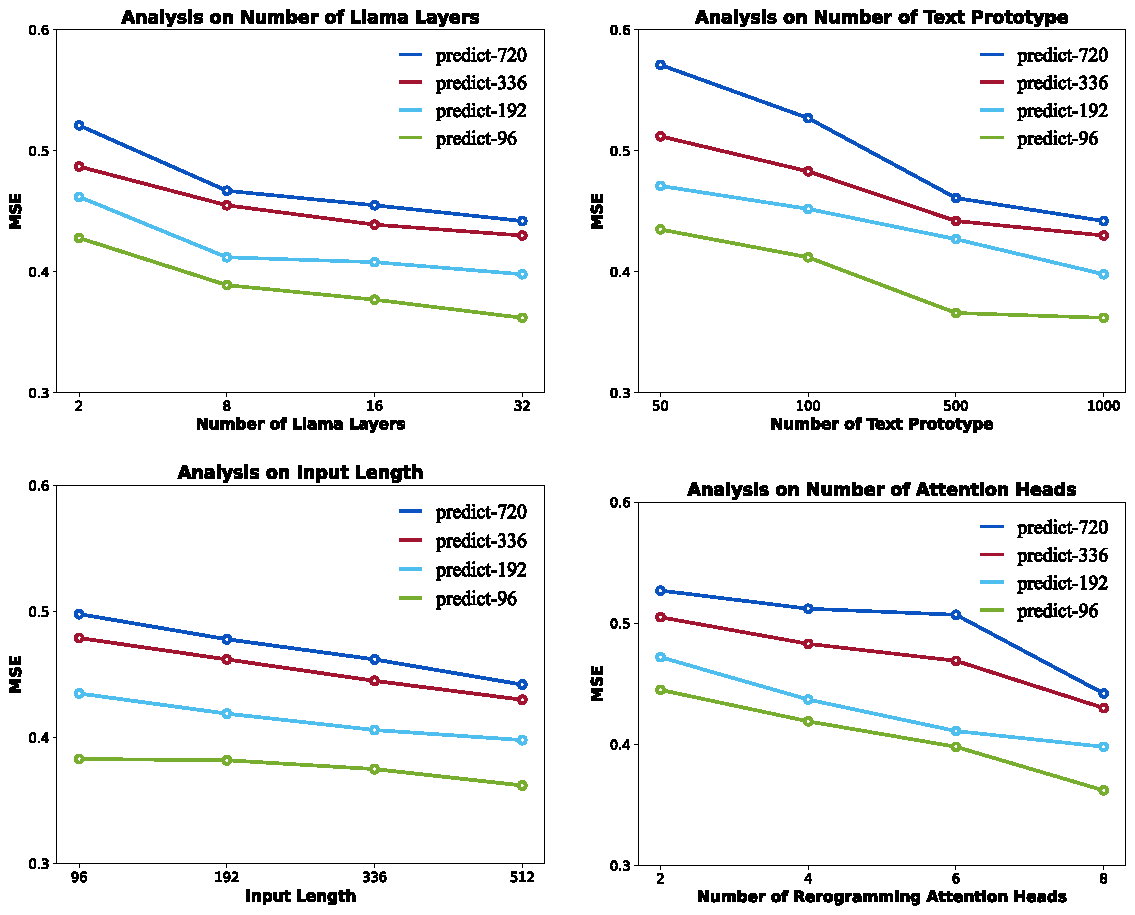
\includegraphics[width=0.95\columnwidth]{figures/sensitivity.pdf}}
	\caption{Analysis of hyperparameter sensitivity on ETTh1 dataset.}
	\label{fig:visual_sensitivity}
\end{center}
\vspace{-25pt}
\end{figure*}